% !Mode:: "TeX:UTF-8"
\chapter{系统详细设计与实现}

上一章从宏观上介绍了本系统的设计,这一章从微观出发,着重介绍中心路径提取模块的设计与实现。

在\ref{afmm-3D}节中讨论了3D中心路径提取算法的原理,这里,我们来看具体实现。
\section{数据结构说明}

从底层的数据结构说起。DARRAY是一个动态数组,它可以在需要的时候动态扩展,并且它支持数据随机删除,类STACK继承自DARRAY。这个数据结构在实现里面保存点的时候很有用,图\ref{darray_class}是类图:
\begin{figure}[h!]
    \centering
    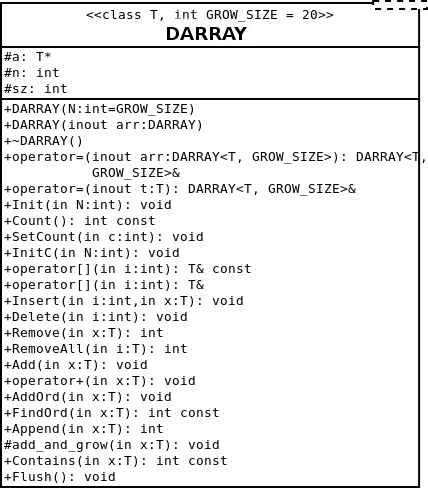
\includegraphics[width=300bp]{figure/darray.png}
    \caption{DARRAY类图}
    \label{darray_class}
\end{figure}

还有一个简单的坐标点的类Coord,类图如\ref{coord-class}。
\begin{figure}[h!]
    \centering
    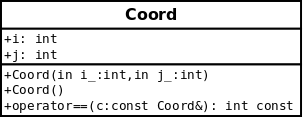
\includegraphics[width=214bp]{figure/coord.png}
    \caption{Coord类图}
    \label{coord-class}
\end{figure}

FIELD是一个模板类,它在逻辑上是一个二维矩阵。里面可以储存各种类型的变量。这个类是很关键的一个类,增强快速行进法处理的二维数据都是这个类的实例。
\begin{figure}[h1]
    \centering
    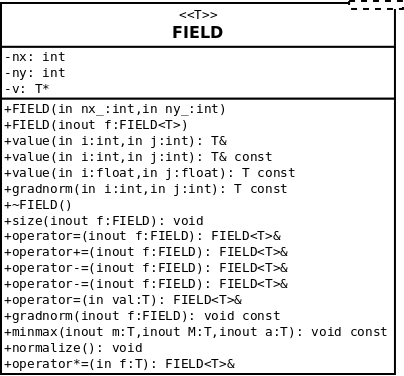
\includegraphics[width=300bp]{figure/field.png}
    \caption{FIELD类图}
    \label{field_class}
\end{figure}

前面有讲到,快速行进法中使用了一个标志$f_{ij}$(参看第\ref{pseudocode}节)。这个标志的实现是一个FLAGS类,它继承自FILED<int>。FLAGS有可能的值有几种,如代码\ref{flag-type}所示:
其中NARROW\_BAND表示BAND类型的点,它的值依然在演化中,也就是窄带上的点。ALIVE是KNOWN类型的点,它的值已经确定,即窄带后面已知点集($A^n$)里面的点。FAR\_AWAY就是INSIDE点,它的值目前还是未知的,即未知区域里面的点。还有一个EXTREMUM,这是一种特殊的已知点,他不仅是已知点,还是极值点。
\begin{lstlisting}[
    language={C},
    caption={FLAGS的类型},
    label={flag-type},
]
enum FLAG_TYPE {
    NARROW_BAND,
    ALIVE,
    FAR_AWAY,
    EXTREMUM
}
\end{lstlisting}

FLAGS的类图如图\ref{flags-class}所示。
\begin{figure}[h!]
    \centering
    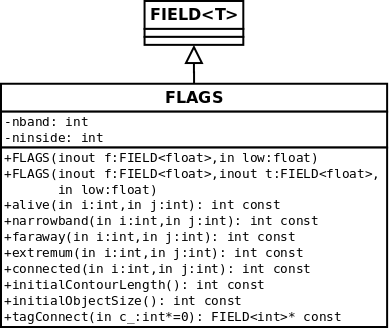
\includegraphics[width=300bp]{figure/flags.png}
    \caption{FLAGS类图}
    \label{flags-class}
\end{figure}

然后就是具体算法部分的快速行进法的类以及增强快速行进法的引擎类,分别是FastMarchingMethod和ModifiedFastMarchingMethod。
快速行进法的类中维护了一些算法需要的信息,最重要的就是一条窄带(即类图中的map),物体的距离变换域(f)以及标志域(flags)。增强快速行进法的类继承自快速行进法。它里面增加了参数化的边界属性(count),如第\ref{afmm-3D}节中讨论的,这个属性通过阈值划分,可以得到骨架。这两个类的类图如\ref{fmm-mfmm-class}(只展示了部分属性)。
\begin{figure}[h!]
    \centering
    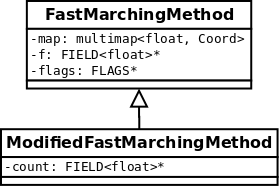
\includegraphics[width=210bp]{figure/fmm_mfmm.png}
    \caption{FastMarchingMethod和ModifiedFastMarchingMethod类图}
    \label{fmm-mfmm-class}
\end{figure}

此外还有一个很重要的类就是VOLUME类,这个类在逻辑上是一个立方阵,存储3D物体的体数据。它可以读取,修改,保存体数据。由于该算法需要将体数据分割成一片一片,在二维上处理,所以它还支持体数据的切片,拼接等功能。
VOLUME的类图如图\ref{volume-class}所示:
\begin{figure}[h!]
    \centering
    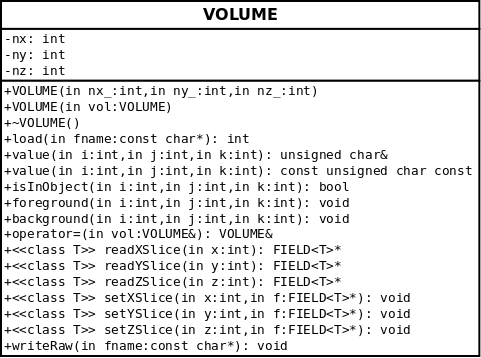
\includegraphics[width=340bp]{figure/volume.png}
    \caption{VOLUME类图}
    \label{volume-class}
\end{figure}

最后,用于提取3D中心路径的是SkelExtractor类,这个类通过调用快速行进法,生成3个坐标轴方向的骨架群,然后求交集,同时还提供有从文件读取体数据,保存体数据及中间过程的骨架群数据的功能。类图如\ref{skelextractor-class}:
\begin{figure}[h!]
    \centering
    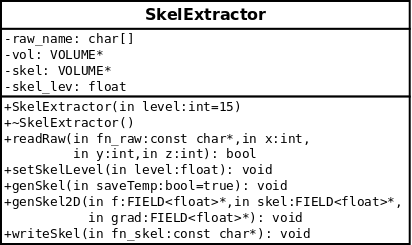
\includegraphics[width=300bp]{figure/skelextractor.png}
    \caption{SkelExtractor类图}
    \label{skelextractor-class}
\end{figure}

\section{功能设计说明}
3D中心路径提取模块主要功能是提取三位物体的中心路径,这是由SkelExtractor类的实例实现的。上一章提到SkelExtractor类的主要功能,下面看一下数据流图,通过数据流图可以看出算法的整体过程。如图\ref{dataflow}。
\begin{figure}[h!]
    \centering
    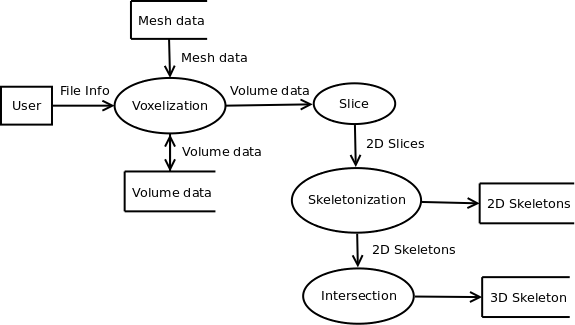
\includegraphics[width=400bp]{figure/dataflow.png}
    \caption{3D中心路径提取算法数据流图}
    \label{dataflow}
\end{figure}
我们接受用户输入的文件信息,会选择读取体数据或者面数据,项目提供了一个十分简陋的脚本来将面数据转化为体数据,我们的后续工作主要是基于体数据的。然后切片,对每个切片求骨架,最后将骨架群求交集。

\subsection{体素化}
项目提供了一个很简单的python脚本用来将mesh格式的面数据转换为体数据。我们使用的体数据是raw形式的,不携带任何其他信息。
\begin{figure}[h!]
    \centering
    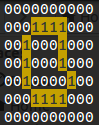
\includegraphics[width=90bp]{figure/connected_boundary.png}
    \caption{连通边界示意图}
    \label{connected-boundary}
\end{figure}
该脚本读取obj格式的网格文件的所有的点并且存储下来,这里我们使用在这个过程中可以确定整个3D空间的大小(点坐标中各个轴坐标的最大值,比如$max_x$、$max_y$、$max_z$)。对于每一个坐标值$z$,可以得到该层上边界点的坐标,我们构造出一个长宽为$max_x$和$max_y$平面$Z$,在分辨率保证的前提下,这个平面上的边界是连通的。比如图片\ref{connected-boundary}。所以我们可以简单的从左上角开始遍历整个整个平面$Z$,如代码\ref{voxelization-code}所示,src是构造的平面,s是体素化后的平面。对于每个点我们处理他的上下左右点。这样能保证不会突破边界到物体内部。这样得到每一个平面的体素化结构,然后组合起来就可以得到体数据。
\begin{lstlisting}[
    language={Python},
    caption={体素化代码},
    label={voxelization-code},
]
def voxelize(cur = (0, 0)):
    todo = []
    x, y = cur
    global src, s
    if s.at(x, y) is 0 or src.at(x, y) == 1 or src.at(x, y) is False:
        return
    
    todo.append((x, y))
    while todo:
        x, y = todo.pop()
        s.set(x, y, 0)
        for (i, j) in [(x-1, y), (x, y-1), (x+1, y), (x, y+1)]:
            if s.at(i, j) == 1 and src.at(i, j) is 0: # False == 0 is True
                todo.append((i, j))
\end{lstlisting}

当然这个方法有两个劣势,这个还待后续改进:
\begin{enumerate}
    \item 原始面数据要足够精细,即分辨率要达到一定程度才能保证边界的连续性;
    \item 不能处理截面是环状的物体;
\end{enumerate}

\subsection{分片}
分片原理很简单,由于我们的体数据存储在一段unsigned char的内存里面。只要精确得计算每个切片平面的点在体数据里面的位置就能直接读取出来构造平面,如代码\ref{slicing-code}是取垂直与$z$轴的平面。
\begin{lstlisting}[
    language={C},
    caption={切片代码},
    label={slicing-code},
]
inline const unsigned char VOLUME::value(int i, int j, int k) const
{
    ... 一些合法性检查代码 ... 
    return *(v + k*nx*ny + j*nx+i);
}

template <class T>
FIELD<T>* VOLUME::readZSlice(int z)       //read z-th layer of z axis
{
    FIELD<T>* slice = new FIELD<T>(nx, ny);
    T* data = slice->data();
    for (int row = 0; row < ny; row++)
    {
        for (int col = 0; col < nx; col++)
        {
            T cur = (value(col, row, z) == 0) ? FG_VALUE : BG_VALUE;
            *data++ = (T)cur;
        }
    }
    return slice;
}
\end{lstlisting}

\subsection{2D骨架提取}
如第\ref{technique}节所说的,2D骨架生成是有增强快速行进法完成的。本项目中实现为ModifiedFastMarchingMethod类。类演化的过程为由execute实现,这个过程中通过init\_count函数来初始化边界参数(即\ref{technique}节中提到的$U$值)。init\_count中先使用一个栈将所有的窄带点保存起来。然后从栈中取栈顶元素为参数化边界的起点。如果栈顶元素是编过号的,继续取栈顶元素,否则的话我们对这个点进行编号,并且将它上下左右四个相邻点中的窄带点再次压栈。这样就可以沿着边界(即窄带)单调得为边界赋予$U$值。

初始化边界完成之后就开始演化,演化调用父类(FastMarchingMethod)的函数execute函数进行演化,函数中会调用diffuse函数进行一次具体的演化过程。在diffuse函数中,执行了以下4步:
\begin{enumerate}
    \item 在窄带中找到最小的距离变换值的点;
    \item 将这个点的标志设置为已知的;
    \item 找到所有待更新的相邻点(不是已知点即可)加到窄带中,这个时候会更新边界参数化的值;
    \item 更新这个点的相邻点的距离变换和标志值。
\end{enumerate}
在更新边界参数化值($U$)的时候,如果该点的4个相邻点中已知点的$U$值最大和最小的相差不大,那么使用已知点的平均$U$值会比较好,若相差太大,那么我们使用第一步中找到的点的$U$值比较好。

循环执行就可以完成整个演化的过程。这个时候我们拿出边界参数化($U$)的域,根据第\ref{section-afmm}中的描述,参数化值相差很大的地方就是骨架点。那么我们先对这个域取梯度,再对梯度进行阈值划分就可以得到骨架。求梯度代码如\ref{threshold-code}:
\begin{lstlisting}[
    language={C},
    caption={边界参数化值域梯度代码},
    label={threshold-code},
]
... 其他 ...
//求梯度的核心代码,cnt是得到的边界参数化域,grad是梯度
for(int j=0;j<grad->dimY();j++)	
    for(int i=0;i<grad->dimX();i++)
    {
        float ux = cnt->value(i+1,j) - cnt->value(i,j);
        float uy = cnt->value(i,j+1) - cnt->value(i,j);
        grad->value(i,j) = max(distance(ux),distance(uy));
    }
...
\end{lstlisting}


\subsection{3D中心路径提取}
切片可以得到对应3个坐标轴的3组切片群,经过上一节就可以得到3个骨架群。
